% Chapter 3

\chapter{EXPERIMENTAL RESULTS AND PERFORMANCE ANALYSIS}

\section{DATASET DESCRIPTION}
In order to avoid the classifier being biased towards the majority classes, it includes a well-balanced and multi-modal dataset with 2,500 samples that are evenly distributed among the five categories of social engineering attacks, with around 500 samples each category, as demonstrated in in~\ref{tab:dataset}.
\begin{table}[h!]
\centering
\caption{Dataset Description}
\label{tab:dataset}
\footnotesize
\renewcommand{\arraystretch}{1.05}
\setlength{\tabcolsep}{3pt}

\resizebox{\textwidth}{!}{%
\begin{tabular}{|p{2.5cm}|p{2cm}|p{9cm}|}
\hline
\textbf{Attack Category} & \textbf{Number of Samples} & \textbf{Description} \\ \hline

Phishing  & 496 & Fraudulent messages aiming to steal sensitive information. \\ \hline
Whaling   & 500 & High-profile targeting attacks aimed at executives. \\ \hline
Pretexting & 518 & Social manipulation using fabricated scenarios to extract data. \\ \hline
Baiting   & 485 & Luring users using fake offers or malicious links. \\ \hline
Legitimate & 501 & Non-malicious samples used as control/normal data. \\ \hline

\textbf{Total} & \textbf{2500} & Balanced dataset across all five classes. \\ \hline

\end{tabular}
}
\end{table}


%
\subsection{Dataset Composition} 
\begin{itemize}
    \item Phishing Attacks: 496 examples of widespread, fraudulent emails that target private information and login passwords.
    \item Whaling Attacks: 500 examples of targeted emails sent to high-value employees and executives.
    \item Pretexting Attacks: 518 instances of dishonest correspondence creating fictitious connections or authority.
    \item Baiting Attacks: 485 samples contain enticing communications with malicious attachments or links.
    \item Legitimate Communications: 501 examples of legitimate communications and real organizational data samples.
\end{itemize}
\subsection{Dataset Distribution} 
Baiting, legitimate, phishing, pretexting, and whaling are the five categories of social engineering attack types that make up the dataset's 2,500 labeled email examples. Each category has between 485 and 518 examples, guaranteeing a nearly balanced class distribution that prevents any one class from overshadowing the learning process. The dataset is separated into four days of incremental learning, in contrast to the usual static dividing of the train and test sets. This simulates a realistic real-world streaming scenario in which fresh data and attack classes are gradually introduced over time.

An 80:20 stratified split is applied separately to the whole pool of examples for each incremental learning day, which consists of both fresh real instances and DAIL-generated synthetic examples from the cluster storage from the day before. A bias toward majority classes in the assessment process is prevented by the stratified split, which guarantees that the class distribution in both the training and test sets appropriately reflects the distribution of active courses for that specific day. The daily distribution is as follows:

\begin{table*}[h]
\centering
\caption{Dataset Distribution}
\label{tab:dataset_distribution}
\resizebox{\textwidth}{!}{
\begin{tabular}{|c|c|c|c|c|c|c|}
\hline
\textbf{Day} & \textbf{Classes Active} & \textbf{New Samples} & \textbf{Augmented} & \textbf{Total Pool} & \textbf{Train (80\%)} & \textbf{Test (20\%)} \\ \hline
Day 1(baiting,phishing,legitimate) & 3 & 700 & 0   & 700  & 560 & 140 \\ \hline
Day 2(baiting,phishing,legitimate,whaling) & 4 & 450 & 180 & 630  & 504 & 126 \\ \hline
Day 3(baiting,phishing,legitimate,whaling,pretexting) & 5 & 576 & 220 & 796  & 636 & 160 \\ \hline
Day 4(baiting,phishing,legitimate,whaling,pretexting) & 5 & 775 & 348 & 1,123 & 898 & 225 \\ \hline
\textbf{Total} & -- & \textbf{2,501} & \textbf{748} & \textbf{3,249} & \textbf{2,598} & \textbf{651} \\ \hline
\end{tabular}
}
\end{table*}

The per-class sample composition on each day mentioned in ~\ref{tab:dataset_distribution}.  represents three different scenarios that the incremental system needs to deal with. In the first scenario, a class receives new real samples and new samples from previous days, which gives a strong training example. In the second scenario, a class receives no new real samples but receives DAIL-augmented samples, which is the most important scenario for preventing catastrophic forgetting, which happens on Day 2 for Baiting and Phishing and on Day 3 for Legitimate and Whaling. In the third scenario, a new class emerges for the first time with only real samples and no augmentation history, which happens on Day 2 for Whaling and on Day 3 for Pretexting.
\subsection{Feature Representation} 
Text Modality:Email body and subject line content transformed into 300-dimensional vectors by using TF-IDF weighting and subsequent matrix factorization.\\
URL Modality:URLs are extracted and represented as 68-dimensional feature vectors that encode syntactic characteristics, domain information, and structural patterns.\\
%BDDs – directed acyclic graph of Boolean expressions. If the variables occur in the same ordering on all paths from root to leaves, we call this OBDD.
%Example: $t=(x_1\&y_1)|(x_2\&y_2)$
%Shannon expansion of t in order x1,y1,x2,y2

%  $t            =x_1\to t_1,t_{01}$

%  $t_1        =y_1\to 1,t_{01}$

%  $t_{01}   =x_2\to t_{011},0$

%  $t_{011} =y_2\to 1,0$
\section{ECOSYSTEM}
\subsection{Hardware Configuration} 
Google Colab’s free-tier runtime provides the following hardware
configuration, which was used throughout model development:
\begin{itemize}
    \item \textbf{RAM:} 16 GB System memory 
    \item \textbf{Storage:}Google Drive integration for accessing datasets and saving model checkpoints.
    \item \textbf{Computational Device:} CPU-based processing.
    \item \textbf{Execution Environment:}Cloud-based runtime with automatic
session management
    
\end{itemize}

\subsection{Software Environment}
The entire system was developed using Python in the Google Colab
environment, supplemented with essential machine learning libraries. The main software components used :
\begin{itemize}
    \item \textbf{Programming Language:} Python 3.8.10

    \item \textbf{Machine Learning Libraries:} scikit-learn 1.1.3, NumPy 1.23.5, Pandas 1.5.3
    \item \textbf{Data Processing:} Scikit-learn preprocessing and feature scaling utilities.
    \item \textbf{Development Environment:} Jupyter Notebook on Google Colab (cloud-based, CPU instances)
\end{itemize}

\section{EXPERIMENTS CONDUCTED}
\subsection{Incremental Learning Scenario Design}
The data was divided into four sequential pieces, each representing four business days, in order to more closely resemble a real-world example of incremental learning, when social engineering attacks change over time and new attack classes appear gradually. A fresh collection of examples is provided every day, and starting on Day 3, new attack classes that weren't there in the days before start to appear. This is done specifically to assess the model's capacity to absorb new information while maintaining the knowledge acquired from earlier days—the stability-plasticity issue that the DAIL method resolves.

\textbf{Day 1 — Initial Training (3 Classes)}\\
Initially, 700 samples from three attack classes—250 legitimate, 250 phishing, and 200 baiting attacks—were used to set up the system. On this day, all of the TF-IDF, SVD, and scaler transformers are applied, and the Stacked Autoencoder is trained from scratch to create the foundation for the feature space. For the duration of the incremental learning period, the frozen transformers from Day 1 will be used on all subsequent days to keep the feature space constant. On Day 1, no augmentation is carried out because there is no prior history to draw from.

\textbf{Day 2 — First Incremental Update (4 Classes)}\\
The second batch introduces 450 new samples — 150 Legitimate and 300 Whaling. Notably, Phishing has zero new real arrivals on Day 2, creating the risk that the updated model will forget previously learned Phishing patterns. DAIL augmentation is applied with $\alpha$, generating some synthetic Phishing samples from Day 1's cluster,few augmented Baiting samples, and few augmented Legitimate samples — totalling augmented samples. These are merged with the new samples to form a sample total training pool.

\textbf{Day 3 — Second Incremental Update (5 Classes)}\\
Test accuracy dropped to 86.25\% following the introduction of Pretexting. Pretexting shares formal, authority-driven language features with both Legitimate and Whaling, causing inter-class confusion. Legitimate had zero new arrivals but was sustained through DAIL-augmented samples, demonstrating effective catastrophic forgetting prevention.

\textbf{Day4 -Third Incremental Update (5 Class)}\\
Test accuracy reached 83.56\% on 225 test samples with all five classes now active. The Day 4 total training pool comprised 1,123 samples — 775 new real samples combined with 348 DAIL-augmented samples drawn from the Day 3 cluster storage. This is the largest training pool across all four days, reflecting the cumulative growth of the incremental system.The day wise data configuration is clearly mentioned in ~\ref{tab:day_wise_config}.

\begin{table}[h]
\centering
\caption{Day wise data configuration}
\label{tab:day_wise_config}
\resizebox{\textwidth}{!}{
\begin{tabular}{|c|c|c|c|c|c|c|c|c|}
\hline
\textbf{Day} & \textbf{New Samples} & \textbf{Classes Active} & \textbf{New Class Introduced} & $\alpha$ & \textbf{Augmented Samples} & \textbf{Total Pool} & \textbf{Train (80\%)} & \textbf{Test (20\%)} \\
\hline
Day 1(baiting,phishing,legitimate) & 700 & 3 & --- & --- & 0 & 700 & 560 & 140 \\
\hline
Day 2(baiting,phishing,legitimate,Whaling) & 450 & 4 & Whaling & 0.40 & 180 & 630 & 504 & 126 \\
\hline
Day 3(baiting,phishing,legitimate,Whaling,pretexting) & 575 & 4 & Pretexting & 0.50 & 220 & 796 & 636 & 160 \\
\hline
Day 4(baiting,phishing,legitimate,whailing,pretexting) & 775 & 5 & None & 0.60 & 348 & 1123 & 898 & 225 \\
\hline
\end{tabular}
}
\end{table}

\subsection{Stacked Autoencoder Experiment}
The first feature extraction was developed to produce deep and dense representations from the raw email text and URL features using a two-step approach: dimensionality reduction and autoencoder-based representation learning.

\textbf{Text Feature Extraction}\\ 
The body and subject of each email were concatenated and preprocessed using lemmatization and regex-based noise removal. A TF-IDF vectorizer with max vocabulary of 2,000 features and unigram-bigram range (1,2) was used to convert the preprocessed text into a sparse matrix. Truncated SVD with 200 components was used to reduce the sparse matrix to a dense 200-dimensional representation. A StandardScaler was used to normalize the output of SVD before passing it to the autoencoder.

The text autoencoder was designed with an architecture of 200$\rightarrow$100$\rightarrow$50$\rightarrow$100$\rightarrow$100$\rightarrow$200, employing \textit{Leaky ReLU} activation functions for all hidden layers and a linear activation for the output layer. The bottleneck layer provides a 50-dimensional encoded representation of the text. The model was trained using the Adam optimizer with Mean Squared Error (MSE) loss for 300 epochs and a batch size of 64.

\textbf{URL Feature Extraction}\\
Four URL characteristics --- URL length, number of dots, number of slashes, and presence of HTTPS --- were manually feature-engineered. In addition, a character-level TF--IDF vectorizer (\texttt{analyzer='char\_wb'}, \texttt{ngram\_range=(3,5)}, \texttt{max\_features=512}) was applied to the raw URL strings, followed by Truncated SVD with 64 components. These features were horizontally stacked to form a 68-dimensional URL feature matrix, which was normalized before training the autoencoder.

The URL autoencoder architecture was 68$\rightarrow$60$\rightarrow$50$\rightarrow$60$\rightarrow$68, again using \textit{LeakyReLU} activation functions, yielding a 50-dimensional encoded URL representation. The model was trained using the same configuration for 300 epochs.

\textbf{Frozen Feature Space}\\
One of the most important design choices is that the autoencoders and all the transformers (TF-IDF, SVD, and scalers) are trained only on Day 1 data, and their weights are set to be frozen for Days 2, 3, and 4. This guarantees that all 124-dimensional feature vectors for all four days are in the same feature space, allowing for a fair comparison and classification across all four days.

The two 50-dimensional outputs are concatenated to create the 100-dimensional output vector
\subsection{Fuzzy-PGDFG Experiment}
The second extracts interpretable, uncertainty-aware features using a fuzzy logic framework applied to manually engineered content features.

\textbf{Manual Feature Engineering}\\ 
Eleven text features are extracted per sample — urgency score, authority score, financial keyword score, credential keyword score, secrecy score, action score, routine score, length score, formality score, time pressure score, and grammar score. Eight URL features are extracted — URL presence, URL length ratio, dot count ratio, digit ratio, HTTPS flag, Shannon entropy, special character ratio, and subdomain count ratio. All 19 features are normalized using StandardScaler.

\textbf{Fuzzy Feature Generation}\\ 
For each class cluster, the Fuzzy-PGFDG computes 16 fuzzy descriptors per sample using Mahalanobis distance, neighborhood density estimation, subspace membership analysis, and entropy-based uncertainty quantification. From these 16, five diverse and non-redundant features are selected:

\begin{itemize}

\item \textbf{Typicality:} Computed as $\exp(-0.5 \times d_M^2)$ where $d_M$ is the Mahalanobis distance --- measures how representative the sample is of its class centroid.

\item \textbf{Density:} Local cluster compactness is encoded by the ratio of class neighbors within the 25th percentile radius.

\item \textbf{Homogeneity:}  Intra-class homogeneity is encoded by the Pearson correlation coefficient between the sample descriptor and class mean.

\item \textbf{Outlier Score:} a modified Z-score that uses the median absolute deviation to identify samples that are close to class borders.

\item \textbf{Fuzzy Entropy:} This measure encodes assignment uncertainty and is the normalized Shannon entropy of the typical/atypical membership pair.

\end{itemize}

2's final output, a 24-dimensional hybrid vector (19 manual + 5 fuzzy), is concatenated with 1's 100-dimensional output to create a 124-dimensional composite feature vector for classification.

\textbf{Data Augmentation Experiment}\\
The DAIL column-alternating augmentation was applied at the start of Days~2, 3, and~4 using the previous day's stored combined 124-dimensional feature matrix as the source pool. For each class cluster, pairs of samples are randomly selected without replacement, and two synthetic samples are generated per pair by alternating feature column values between the two parent samples:

\[
Q_1[j] =
\begin{cases}
S_1[j] & \text{if } j \bmod 2 = 0 \\
S_2[j] & \text{if } j \bmod 2 = 1
\end{cases}
\qquad
Q_2[j] =
\begin{cases}
S_2[j] & \text{if } j \bmod 2 = 0 \\
S_1[j] & \text{if } j \bmod 2 = 1
\end{cases}
\]

This guarantees that all generated samples remain within their parent cluster's feature distribution.The per-class augmentation outcomes across the three augmented days are mentioned in Table ~\ref{tab:per-class-aug}

\begin{table}[h]
\centering
\caption{Per-class augmentation outcomes}
\label{tab:per-class-aug}
\begin{tabular}{|c|c|c|c|p{4.5cm}|}
\hline
\textbf{Day} & \textbf{Class} & \textbf{Prev. Cluster Size} & \textbf{Samples Generated}  \\
\hline
Day 2 & Baiting & 200 & 60 \\
Day 2 & Legitimate & 250 & 60 \\
Day 2 & Phishing & 250 & 60 \\
Day 2 & Whaling & 0 & New class \\

\hline
Day 3 & Baiting & 300 & 60  \\
Day 3 & Legitimate & 210 & 80 \\
Day 3 & Phishing & 60 & 60 \\
Day 3 & Whaling & 300 & 80 \\
Day 3 & Pretexting & 0 & New class\\


\hline
Day 4 & Baiting & 180 & 90 \\
Day 4 & Legitimate & 90 & 40  \\
Day 4 & Phishing & 156 & 78 \\
Day 4 & Whaling & 90 & 40 \\
Day 4 & Pretexting & 300 & 100\\
\hline
\end{tabular}
\end{table}
\subsection{Classifier Training Experiment - ELM}
\textbf{ELM Training}\\

For each day, the ELM was trained on the standardized combined feature matrix. A grid search was performed over dynamically computed $n_{\text{hidden}}$ candidates $\left(\frac{n_{\text{train}}}{6}, \frac{n_{\text{train}}}{4}, \frac{n_{\text{train}}}{3}\right)$ and three activation functions (\textit{sigmoid}, \textit{ReLU}, \textit{tanh}). Output weights were computed analytically using the Moore--Penrose pseudoinverse with $L_2$ regularization $(\lambda = 10^{-2})$. The best configuration was selected using the gap-penalized scoring criterion.

\vspace{0.5em}

\section{PERFORMANCE ANALYSIS}
\subsection{SAE - ELM Analysis} 
First evaluates deep latent feature representations learned using TF-IDF, truncated SVD, and a Stacked Autoencoder (SAE) before ELM classification. With 200 hidden neurons and ReLU activation, the best combination demonstrated 84.67\% accuracy, indicating that encoded representations with lower dimensionality can successfully capture semantic and structural patterns in text and URL feature data. Whereas excessively large hidden layers resulted in reduced generalization, performance was stable for moderate hidden sizes (100–300 neurons). The comparatively poorer performance on related attack classes suggests that deep feature representations might not be enough to capture uncertainty and class overlap, even clearly has robust representation learning capabilities.

\begin{table}[h]
\centering
\caption{Performance Comparison of ELM Configurations 1}
\label{tab:elm_pipeline1}
\begin{tabular}{|c|c|c|c|}
\hline
\textbf{Hidden Neurons} & \textbf{Activation Function} & \textbf{Accuracy} & \textbf{Macro F1-Score} \\ \hline
100 & Sigmoid & 0.8493 & 0.85 \\ \hline
150 & Sigmoid & 0.8573 & 0.86 \\ \hline
200 & ReLU    & 0.8467 & 0.84 \\ \hline
300 & ReLU    & 0.8387 & 0.84 \\ \hline
\end{tabular}
\end{table}

With 150 hidden neurons and Sigmoid activation, the best combination was found, with 95.60\% accuracy and a macro F1-score of 0.9601 as mentioned in ~\ref{tab:elm_pipeline1}. This clearly demonstrated a huge improvement over first due to the usage of fuzzy features.

\subsection{Original Features+Fuzzy Features - ELM Analysis} 

For behavioral features that are manually created and enhanced using fuzzy membership descriptors, shows itself to be a reliable classifier. The concatenated model that combined fuzzy attributes significantly increased the baseline model's accuracy to 95.60\% from 92.40\%. Particularly in semantically related assault types like phishing and whaling, the addition of Typicality, Density, Homogeneity, Outlier Score, and Fuzzy Entropy significantly aided in class separation. The ELM classifier's hyperparameter optimization showed that a modest number of hidden neurons (100–300) with sigmoid or ReLU activation functions performed best. The experiment unequivocally demonstrates that using fuzzy modeling to manage uncertainty enhances generalization and robustness in the detection of social engineering attacks.
\begin{table}[h]
\centering
\caption{Performance Comparison of ELM Configurations 2(Hybrid Model)}
\label{tab:elm_pipeline2}
\begin{tabular}{|c|c|c|c|}
\hline
\textbf{Hidden Neurons} & \textbf{Activation Function} & \textbf{Accuracy} & \textbf{Macro F1-Score} \\ \hline
100 & Sigmoid & 0.940 & 0.9225 \\ \hline
150 & Sigmoid & 0.9450 & 0.9401 \\ \hline
200 & ReLU    & 0.9560 & 0.9563 \\ \hline
300 & ReLU    & 0.9340 & 0.9242 \\ \hline
\end{tabular}
\end{table}

As mentioned in ~\ref{tab:elm_pipeline2} The best-performing configuration was achieved with 150 hidden neurons using Sigmoid activation, yielding 95.60\% accuracy and a macro F1-score of 0.95, demonstrating a substantial improvement over 1 due to the integration of fuzzy features.

\subsection{Day-wise Incremental Performance - ELM}
The proposed system was evaluated across four incremental learning days using the Extreme Learning Machine (ELM) as the primary classifier. The ELM was trained on the 124-dimensional combined feature vector produced by the dual-pipeline feature extraction framework — 100 dimensions from the Stacked Autoencoder and 24 dimensions from the Fuzzy-PGFDG. For each day, a gap-penalized hyperparameter search was conducted to identify the optimal hidden layer size and activation function. The complete day-wise performance is summarized below in table ~\ref{tab:daywise_incremental_analysis}

\begin{table}[h]
\centering
\caption{Day-wise Incremental Analysis}
\label{tab:daywise_incremental_analysis}
\small
\setlength{\tabcolsep}{4pt}
\begin{tabular}{|p{4.2cm}|c|c|c|c|c|}
\hline
\textbf{Batch (Day)} & \textbf{Training} & \textbf{Test} & \textbf{ELM Train} & \textbf{ELM Test} & \textbf{Train-Test} \\
 & \textbf{Samples} & \textbf{Samples} & \textbf{Accuracy (\%)} & \textbf{Accuracy (\%)} & \textbf{Gap (\%)} \\
\hline
Day 1 (baiting, phishing, legitimate) & 560 & 140 & 99.64 & 92.86 & 6.78 \\
\hline
Day 2 (baiting, phishing, legitimate, whaling) & 453 & 114 & 99.60 & 88.89 & 10.71 \\
\hline
Day 3 (baiting, phishing, legitimate, whaling, pretexting) & 609 & 153 & 97.80 & 86.25 & 11.55 \\
\hline
Day 4 (baiting, phishing, legitimate, whaling, pretexting) & 898 & 225 & 96.55 & 83.56 & 12.99 \\
\hline
\end{tabular}
\end{table}
\subsection{ELM Hyperparameter Selection Analysis}

\noindent
For each incremental day, the ELM hyperparameter search evaluated all combinations of dynamically computed $n_{\text{hidden}}$ candidates and three activation functions ($\text{sigmoid}$, $\text{relu}$, and $\text{tanh}$) using the gap-penalized scoring criterion.

\begin{equation}
\text{Score} = \text{Test Accuracy} - 0.5 \times \max(0, \text{Gap} - 0.10)
\end{equation}

\noindent
The selection of topologies that strike a compromise between prediction accuracy and generalization capability is encouraged by this criterion, which penalizes any train-test gap more than 10\% by lowering the effective score.

\begin{table*}[h]
\centering
\caption{Gap-Penalized Hyperparameter Selection Across Incremental Days}
\label{tab:gap_penalized_selection}
\resizebox{\textwidth}{!}{
\begin{tabular}{|c|c|c|c|c|c|c|c|}
\hline
\textbf{Day} & \textbf{$n_{\text{hidden}}$} & \textbf{Best $n_{\text{hidden}}$} & \textbf{Act.} & \textbf{Train (\%)} & \textbf{Test (\%)} & \textbf{Gap (\%)} & \textbf{Score} \\ \hline
Day 1(baiting,phishing,legitimate) & 93,140,186  & 186 & tanh    & 99.64 & 92.86 & 6.78  & 0.9286 \\ \hline
Day 2(baiting,phishing,legitimate,whaling) & 75,113,151  & 126 & relu    & 99.60 & 88.89 & 10.71 & 0.8854 \\ \hline
Day 3(baiting,phishing,legitimate,whaling,pretexting) & 101,152,203 & 159 & sigmoid & 97.80 & 86.25 & 11.55 & 0.8548 \\ \hline
Day 4(baiting,phishing,legitimate,whaling,pretexting) & 125,188,251 & 299 & relu    & 96.55 & 83.56 & 12.99 & 0.8206 \\ \hline
\end{tabular}
}
\end{table*}

\noindent
Over the course of the four days,as mentioned in Table ~\ref{tab:gap_penalized_selection} it was observed that while larger values of $n_{\text{hidden}}$ result in training data memorization, lesser values lead to better generalization but worse training accuracy. Instead of selecting the largest candidates, the gap-penalized selector selects intermediate settings that offer the optimal balance between generalization and accuracy. When more attack classes are introduced, the non-linearity in decision boundaries increases, as evidenced by the best activation function shifting from tanh on Day 1 to relu on Days 2 and 4.

\subsection{Complete Tabulation of Results}
The whole day-by-day outcomes of the incremental learning process are summarized in the master table below, along with comprehensive class data as depicted in table ~\ref{tab:daywise_distribution}:

\begin{table*}[h]
\centering
\caption{Day-wise Training Distribution and Incremental Performance}
\label{tab:daywise_distribution}
\resizebox{\textwidth}{!}{
\begin{tabular}{|c|p{6.5cm}|c|c|c|}
\hline
\textbf{Day} & \textbf{Training Set (Class : Samples)} & \textbf{Test Set (Samples)} & \textbf{Training Acc (\%)} & \textbf{Testing Acc (\%)} \\ 
\hline

Day 1 & Baiting: 160, Legitimate: 200, Phishing: 200 (Total: 560) & 140 & 99.64 & 92.86 \\ \hline

Day 2 & Baiting: 48, Legitimate: 168, Phishing: 48, Whaling: 240 (Total: 504) & 126 & 99.60 & 88.89 \\ \hline

Day 3 & Baiting: 144, Legitimate: 64, Phishing: 124, Pretexting: 240, Whaling: 64 (Total: 636) & 160 & 97.80 & 86.25 \\ \hline

Day 4 & Baiting: 180, Legitimate: 112, Phishing: 159, Pretexting: 254, Whaling: 192 (Total: 898) & 225 & 96.55 & 83.56 \\ \hline

\end{tabular}
}
\end{table*}

\begin{figure}[h]
\centering
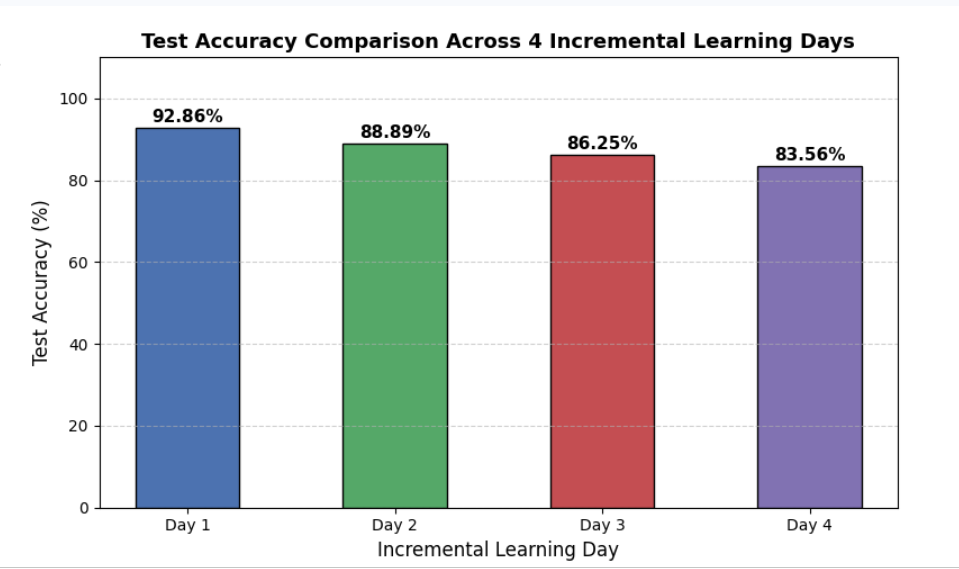
\includegraphics[width=\linewidth]{images/overall_result_chart.png}
\caption{Test Accuracy Comparison Across Four Incremental Learning Days}
\label{fig:test_accuracy_incremental}
\end{figure}

With an increasingly larger dataset that increased from 700 to 1,123 samples over the course of the incremental learning process, the ELM's average test accuracy on all four incremental days was 87.89\%, correctly classifying all five categories of social engineering attacks: baiting, legitimate, phishing, pretexting, and whaling. DAIL augmentation was also found to be a successful method for information retention in the system, as no previously acquired class was completely forgotten during the incremental learning process.